\documentclass[english]{article}
\usepackage[italian]{babel} 
\usepackage[T1]{fontenc}
\usepackage[utf8x]{inputenc}
\usepackage{float}
\usepackage{graphicx}
\makeatletter
\usepackage[a4paper,top=2cm,bottom=2cm,left=2cm,right=2cm]{geometry}
\usepackage{enumitem}
\usepackage{subfig}
\usepackage{amsthm}
\usepackage{amsmath}
\usepackage{epstopdf}
\usepackage{fancyhdr}
\usepackage{booktabs,array}
\newcommand*{\eacc}{\MakeUppercase{è }}

% Pacchetto per la gestione del testo colorato
\usepackage{color}

% Pacchetto che permette l'inserimento di codice Matlab formattato
\usepackage{listings} % inserisce listati di programmi
\definecolor{commenti}{rgb}{0.13,0.55,0.13}
\definecolor{stringhe}{rgb}{0.63,0.125,0.94}
\lstloadlanguages{Matlab}
\lstset{% general command to set parameter(s)
framexleftmargin=4mm,
frame=single,
keywordstyle = \color{blue},% blue keywords
identifierstyle =, % nothing happens
commentstyle = \color{commenti}, % comments
stringstyle = \ttfamily \color{stringhe}, % typewriter type for strings
showstringspaces = false, % no special string spaces
emph = {for, if, then, else, end},
emphstyle = \color{blue},
firstnumber = 1, % numero della prima linea
numbers =left, %  show number_line
numberstyle = \tiny, % style of number_line
stepnumber = 5, % one number_line after stepnumber
numbersep = 5pt,
language = {Matlab}, % per riconoscere la sintassi matlab
extendedchars = true, % per abilitare caratteri particolari
breaklines = true, % per mandare a capo le righe troppo lunghe
breakautoindent = true, % indenta le righe spezzate
breakindent = 30pt, % indenta le righe di 30pt
}




\hyphenation{italian}
\lhead{Progettazione Sistemi di controllo}
\rhead{Homework 1}

%\linespread{1.3}

%\@ifundefined{showcaptionsetup}{}{%
% \PassOptionsToPackage{caption=false}{subfig}}
%\usepackage{subfig}
\makeatother

\usepackage{babel}

\begin{document}
\begin{titlepage} 

\begin{center}
\begin{Large} \textbf{UNIVERSITA' DEGLI STUDI DI PADOVA} \\
 \end{Large} \vspace{1cm}

\begin{Large} \textsc{Corso di Robotica Autonoma }\end{Large}
\par\end{center}

\begin{center}
\begin{Large}\textsc{Esperienza 1}\\
 \end{Large}
\par\end{center}

\begin{center}
\vspace{2cm}
\begin{figure}[!htb]
\centering 
\includegraphics[width=8cm]{unipd}\\
 
\end{figure}

\par\end{center}

\begin{center}
\vspace{2cm}
 \begin{Large}
 GRUPPO 11: \\
 Marco Bertagnoli \\ 
 Matteo Mastellaro \\ 
 Angelo Trevisol\\
 \end{Large} \vspace{2cm}
 \begin{Large} Anno Accademico 2015-2016 \end{Large} 
\par\end{center}

\end{titlepage}

\tableofcontents
\newpage

\section{Panoramica}
L'obiettivo generale di questa esperienza è implementare un software che sia in grado di guidare un robot Lego Nxt all'interno di una mappa, da una certa posizione detta "Start" ad una posizione finale, detta "Goal", in diversi scenari che racchiudono diverse difficoltà. Tale software sarà implementato in linguaggio C++, orientato agli oggetti, e la comunicazione con il robot sarà effettuata attraverso ROS (Robot Operating System) i cui dettagli verranno discussi più avanti.

\subsection{Mappa} La mappa in cui il robot può muoversi è una matrice su sfondo verde, composta da nxm quadrati, individuati da linee bianche, in cui all'interno di ciascuno è possibile trovare un ostacolo, individuato da un cono. Il movimento all'interno della mappa è consentito soltanto nelle direzioni Nord, Sud, Est e Ovest, ovvero non è consentito il movimento diagonale. Una rappresentazione della mappa presente in Laboratorio è rappresentata in Figura \ref{fig: mappa_gen}.
\begin{figure}[!h]
\centering
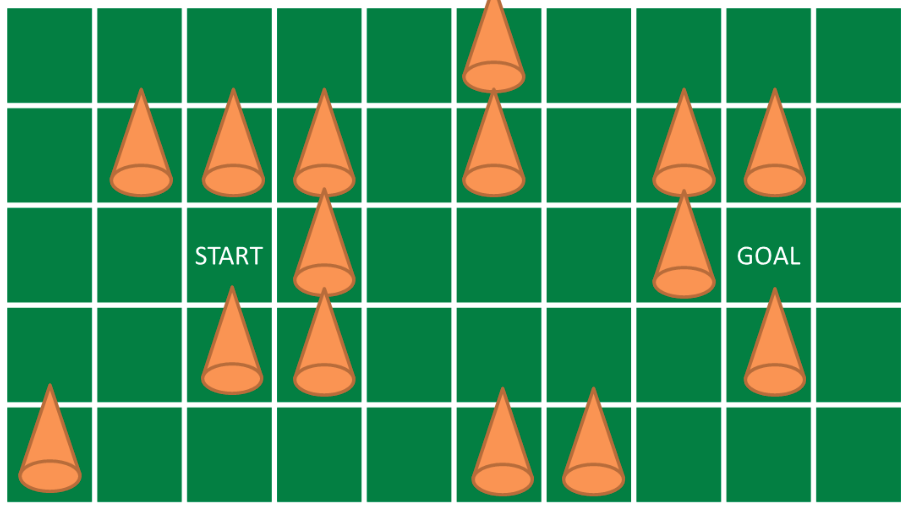
\includegraphics[width=0.35\textwidth]{mappa_generale}
\caption{Rappresentazione della mappa presente in laboratorio.}
\label{fig: mappa_gen}
\end{figure}

\subsection{Scenario} La navigazione del robot Nxt sarà effettuata in diversi scenari. In un primo scenario la mappa non presenterà ostacoli; questo è il caso più semplice infatti l'algoritmo che guida il robot non dovrà preoccuparsi di individuare eventuali presenze di ostacoli, ma potrà liberamente muoverlo verso l'obiettivo. 

In un secondo scenario, la mappa presenta degli ostacoli fissi, la cui posizione viene fornita in anticipo al robot, in modo che quest'ultimo possa calcolare il percorso prima di iniziare a muoversi. Una volta che il percorso è stato valutato, il robot dovrà soltanto seguire il tracciato. Questa seconda situazione presenta una difficoltà aggiuntiva legata alla posizione degli ostacoli, che per esempio potrebbero portare il robot in una strada senza uscita.

Infine l'ultimo e il più complesso scenario, nel quale il robot non conosce in anticipo la presenza degli ostacoli (che potrebbero anche spostarsi nel tempo) e dunque è costretto, passo dopo passo, a rilevare gli ostacoli attraverso i sensori e valutare di volta in volta il percorso per arrivare all'obiettivo. 

Una buona pratica per passare informazioni al robot sul tipo di scenario che esso deve affrontare, è quella di passare attraverso un file con estensione ".yaml". Dunque la scrittura del file "mappa.yaml" è stata fatta in questo modo:
\begin{verse}
$\%$YAML:1.0\\
Dimensione: \\
 altezza: 5\\
 lunghezza: 10\\ 
Inizio: \\
 x: 5\\
 y: 2\\
Arrivo:\\
 x: 8\\
 y: 2\\
Ostacoli:\\
 numero$\_$ostacoli:0 $\#$15\\
 x:[] $\#$ [0, 2, 3, 3, 3, 2, 1, 5, 6, 5, 5, 8, 7, 7, 8]\\
 y:[] $\#$ [0, 1, 1, 2, 3, 3, 3, 0, 0, 3, 4, 1, 2, 3, 3]\\
DrawMap: 1\\
TerzoPunto: 1\\
\end{verse}
In questo script si è specificato nel campo \textit{Dimensione} rispettivamente il numero di righe e di colonne della matrice-mappa, in \textit{Inizio} e \textit{Fine} rispettivamente le celle di start e goal in coordinate cartesiane, e nel campo \textit{Ostacoli} vengono specificati il numero e le posizioni degli ostacoli all'interno della mappa. 
Con il campo \textit{DrawMap} è possibile attraverso il valore 1, comunicare al software di voler aggiungere una mappa grafica, creata mediante il tool \textit{Opencv}, che visualizza graficamente i progressi del robot, ad ogni istante temporale. Il suo funzionamento cerrà chiarito nella sezione di test in laboratorio.
Per concludere, con il valore 1 è possibile attivare il campo \textit{TerzoPunto}, con cui si comunica al robot che la mappa è a priori ignota, ed è dunque necessario attivare i sensori ad ultrasuoni per riconoscere gli ostacoli e valutare il percorso ad ogni passo (ultimo scenario descritto).

\subsection{Robot Lego NXT}
Il robot Lego NXT in Figura \ref{fig: nxt} include gli strumenti e i sensori per affrontare l'esperienza negli scenari descritti in precedenza. Nel nostro caso, il robot è dotato di :
\begin{itemize}
\item \textbf{Due ruote motrici} azionate elettricamente, che permettono al robot di avanzare, retrocedere, e ruotare su se stesso.
\item \textbf{Sensore ad ultrasuoni} per rilevare la presenza di ostacoli nella mappa, esso è montato su supporto che può ruotare di 360 gradi, grazie ad un apposito motore elettrico.
\item \textbf{Sensore di luce} per rilevare il colore del terreno, utile per individuare quadrati (individuati da linee bianche) sulla matrice verde.
\item \textbf{Odometria}: è uno strumento molto utile che il robot fornisce, con questo infatti esso, sommando i molteplici spostamenti relativi, tiene traccia dello spostamento globale effettuato, rispetto alla sua posizione di partenza. In questo modo è possibile sapere, istante per istante la posizione del robot e la rispettiva orientazione rispetto a quelle di partenza.
\end{itemize}
\begin{figure}[!h]
\centering
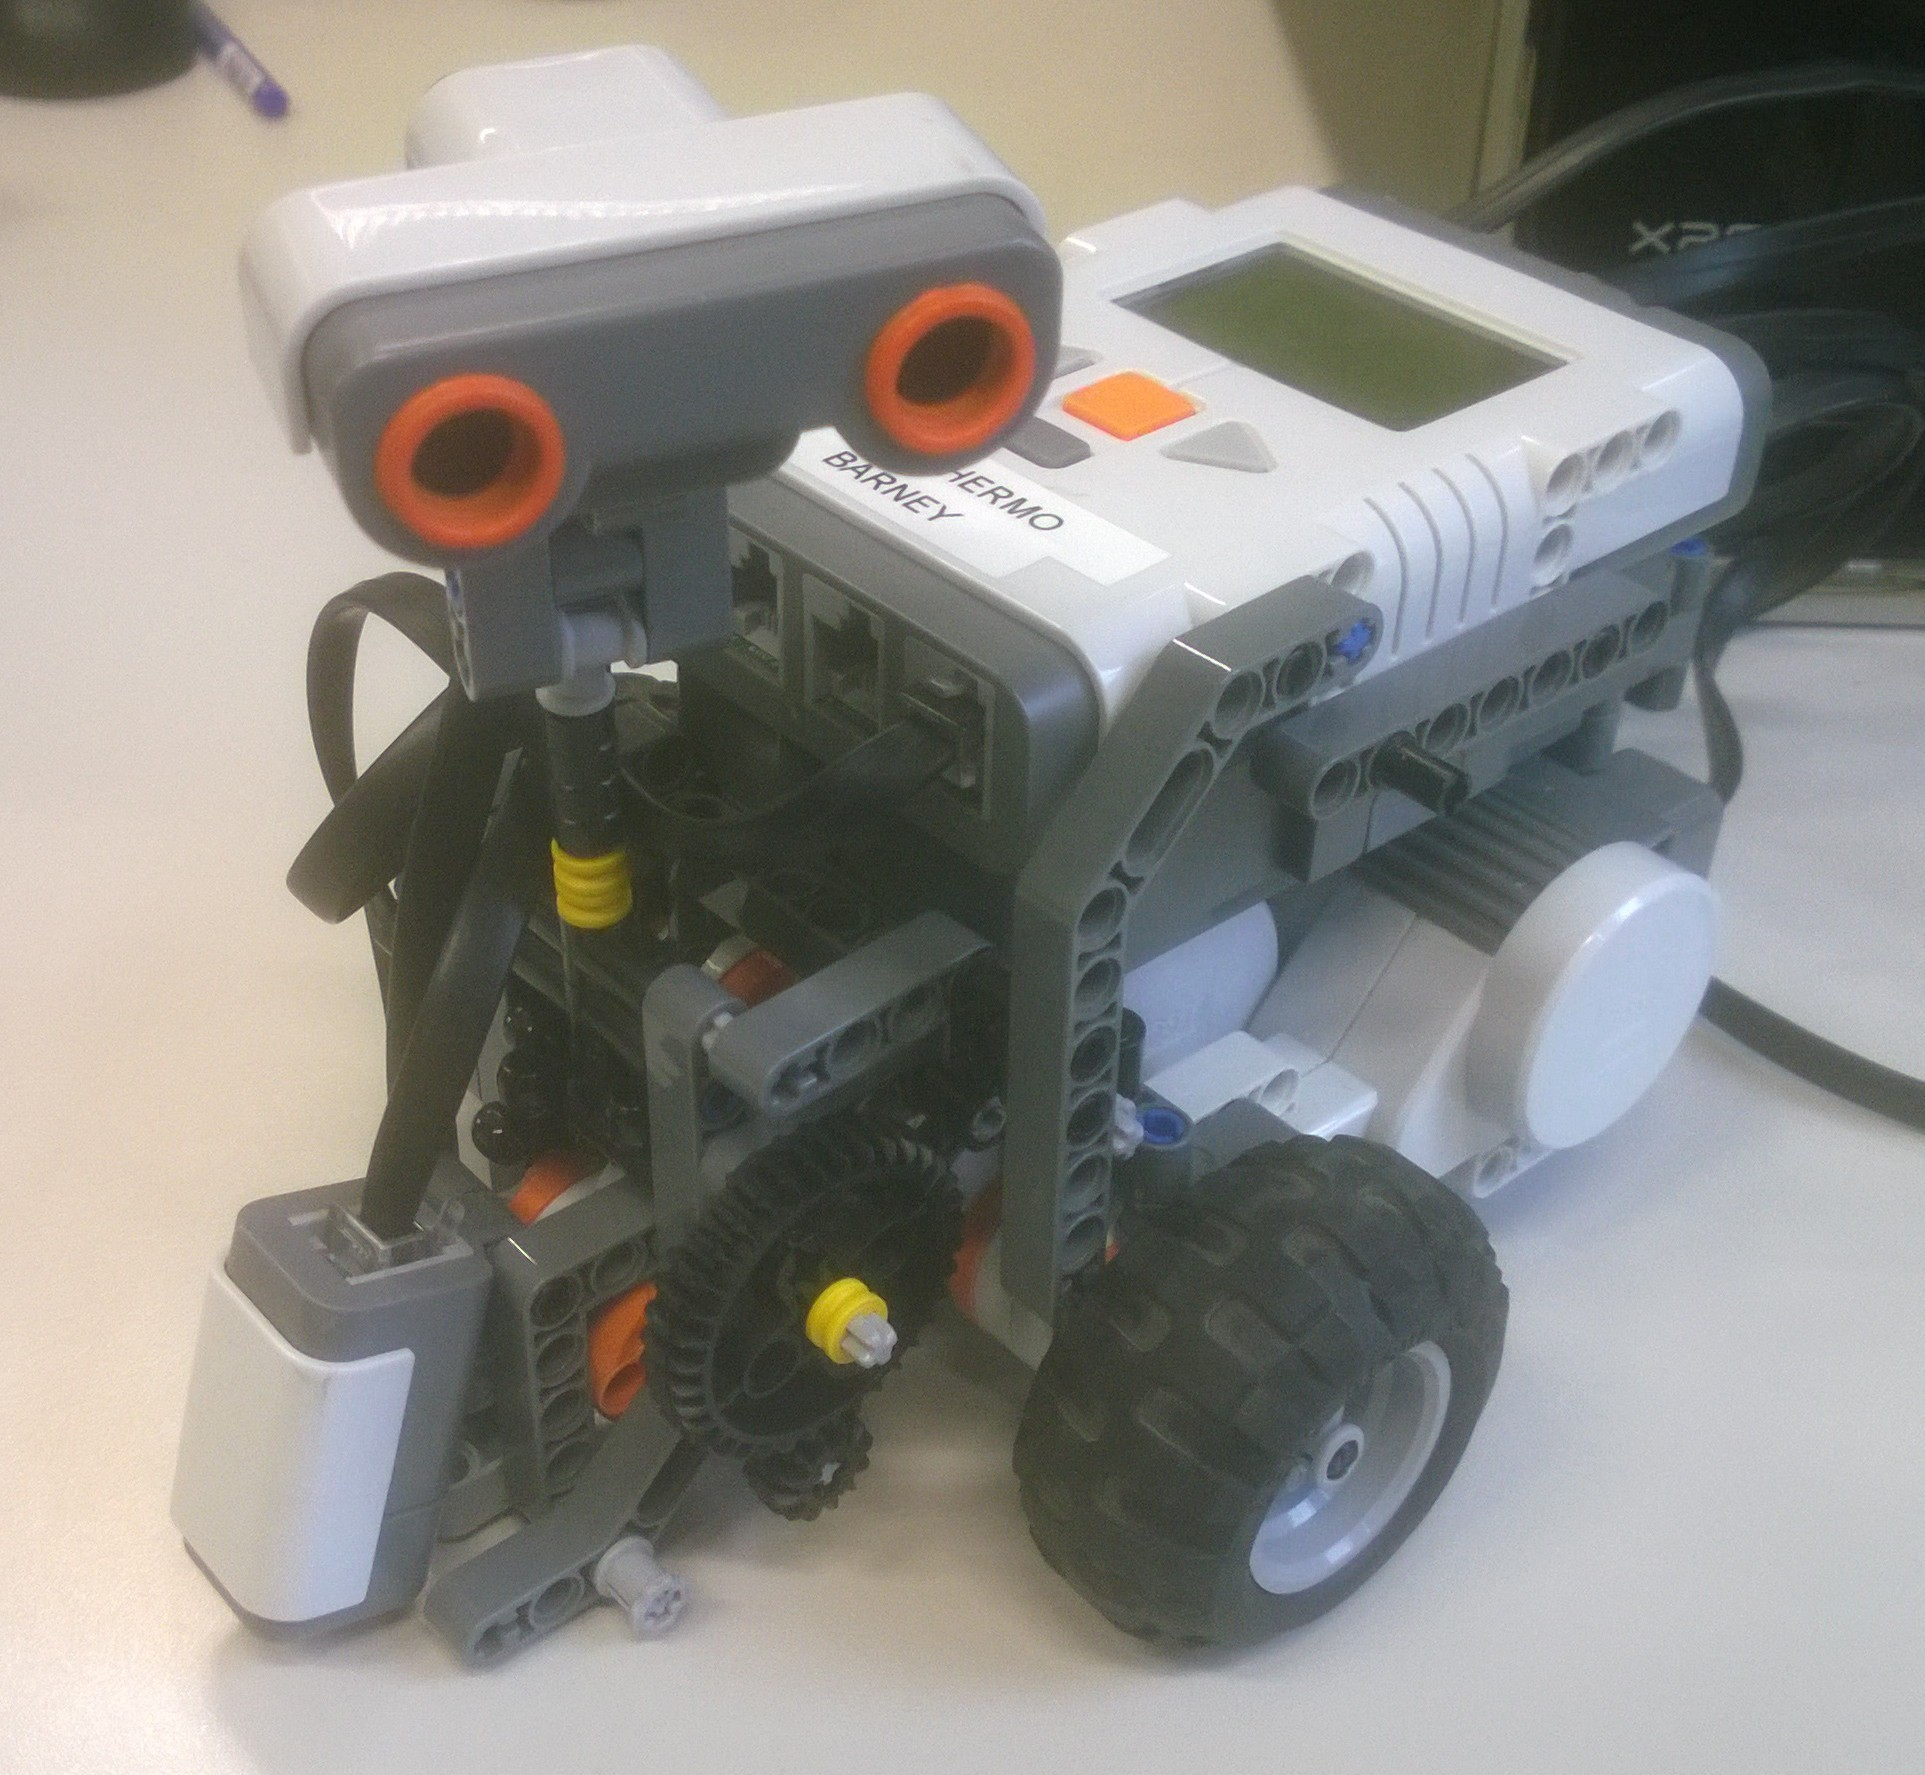
\includegraphics[width=0.3\textwidth]{nxt}
\caption{Mettere una foto con due ruote !!!}
\label{fig: nxt}
\end{figure}


\section{Realizzazione del Software}
Come già accennato nella sezione introduttiva, l'implementazione degli algoritmi viene eseguita in C++, mentre l'interfacciamento con il robot viene fatto mediante la utility ROS. Quest'ultimo si basa sulla comunicazione di diversi nodi, che vengono creati in fase di implementazione del software. Dunque per lanciare il software si è innanzitutto creato un file "launcher" (chiamato "esperienza1.launch") che si occupa di avviare tre nodi principali che sono stati individuati, ovvero:
\begin{itemize}
\item \textbf{Robot}: si occupa della gestione dei movimenti del robot;
\item \textbf{Mapping}: si occupa della creazione e della gestione della mappa;
\item \textbf{Navigation}: si occupa dell'algoritmo di navigazione che porta il robot dallo start al goal.
\end{itemize}
Come si può intuire ciascun nodo per gestire il suo task, ha bisogno di informazioni che derivano da altri nodi, perciò questi ultimi necessitano di comunicare costantemente durante l'esecuzione. Tali comunicazioni verranno approfondite più avanti, ma avvengono attraverso "servizi" di diverso tipo, che vengono richiesti e forniti da ciascun nodo che, all'occorrenza farà da client o da server. La creazione e la gestione dei nodi è stata realizzata attraverso una classe dedicata per ciascun nodo. [AGGIUNGERE SCHEMA DI COMUNICAZIONE DEI NODI (RQTPLOT]

\subsection{Mappa (angelo)}
Per la creazione della mappa è stata definita la classe “Cella” che contiene un intero che rappresenta la distanza dall’arrivo, un booleano che indica se la cella è occupata da un qualche ostacolo ed infine un altro intero che funge da contatore per la scomparsa automatica del blocco, nel caso i blocchi non siano fissi, così da evitare che la cella resti interdetta per sempre.

È stata poi creata la classe “Mappa” che è una matrice di celle della dimensione della mappa dove dovrà poi muoversi il robot. Una volta creata la matrice, e definita la cella arrivo, viene poi “popolata” cioè vengono assegnate le distanze alle varie celle: inizialmente si assegna a tutte le celle la distanza massima possibile (dette 𝑙 ed 𝑎 le dimensioni della matrice tale valore sarà 𝑙×𝑎), si attribuisce all’arrivo 0 e lo si inserisce in una coda dalla quale si estrae, finche’ ce n’è, il primo elemento e si assegna alle celle adiacenti a quest’ultimo una distanza pari a quella della cella in questione incrementata di un’unità e messe a loro volta nella coda (a patto che queste celle vicine abbiano un peso strettamente maggiore e non siano blocchi). Quando la coda è vuota l’intera mappa è stata popolata. Con questo procedimento non si hanno direzioni privilegiate di esplorazione della mappa ma si procede in maniera spiraliforme e si evita, con la diseguaglianza stretta, di incorrere in loop dovuti ad eventuali percorsi multipli.

Da un’analisi sull’algoritmo risulta una complessità di O(n) con n il numero di celle della matrice mappa.

\subsection{Navigazione (angelo)}
La parte di navigazione è relativamente semplice sfruttando la mappa definita poc’anzi, basta infatti spostarsi verso la cella adiacente che ha il peso minore, a patto di non trovarsi già all’arrivo (ed, ovviamente, restando nella mappa).

Se la cella dove è previsto muoversi risulta occupata da un ostacolo di qualche tipo si provvede ad aggiornare la mappa ed a ricalcolarla.

Ogniqualvolta il movimento verso una nuova cella risulta compiuto viene decrementato il contatore di tutte le celle blocco: questo serve perché se si imbocca un vicolo cieco e mentre si retrocede la strada viene bloccata, dopo un po’ si ritenteranno percorsi prima considerati bloccati.

Questo sistema di navigazione risulta essere molto efficiente poiché’ la scelta del percorso richiede, praticamente, solo un’operazione basilare e le operazioni più complesse di popolamento della mappa avvengono abbastanza di rado ma sono comunque nell’ordine di grandezza della mappa stessa.

Inoltre, a differenza di altri algoritmi tipo A*, questo sistema di esplorazione (sarebbe meglio dire popolamento) anche in caso di investigazione di una strada non ottimale non la esplora completamente

prima di accorgersi che è tale, nel caso peggiore arriverà a metà della stessa da due direzioni differenti. Va tenuto in considerazione però che A* nel caso ottimo è molto più veloce esplorando molte meno strade.
  
  
  
\subsection{Spostamento del robot (matteo)}
Per lo spostamento del robot all'interno della mappa si sono innanzitutto individuati i singoli movimenti necessari a farlo muovere correttamente all'interno dell'ambiente. Si sono isolate 5 azioni:
\begin{itemize}
\item Rotazione;
\item Movimento in linea retta;
\item Avanzamento di una cella;
\item Centramento all'interno della cella;
\item Riceca dei coni.
\end{itemize}

Si è scelto allora di creare una classe (\textit{Navigate\_Nxt}) che ci permettesse di accedere velocemente a tutti questi movimenti in modo da poterli comporre per far spostare il robot all'interno della mappa. La classe prende in ingresso un nodo ros su cui poi andrà a lavorare. Innanzitutto in fase di costruzione va ad iscrivere il nodo a tutti i topic necessari al controllo del robot. Sarà quindi iscritto come publisher ai topic \textit{$\setminus$cmd\_vel} ed \textit{$\setminus$angle} per poter far muovere i motori delle ruote e del giunto centrale, e come subscriber ai topic \textit{$\setminus$odom}, \textit{$\setminus$intensity\_sensor}, \textit{$\setminus$joint\_states} e \textit{$\setminus$ultrasonic\_sensor} per poter raccogliere i dati forniti dai sensori del robot.

\subsubsection{Rotazione}
Il movimento di rotazione del robot è stato implementato nel metodo \textit{Navigate\_Nxt::rotate(char direction)}.\\
Con questo metodo il robot può cambiare il proprio orientamento nella mappa. Si è scelto di utilizzare un sistema di riferimento assoluto. \eacc allora possibile comunicare al robot di girarsi allineandosi con le quattro direzioni parallele ai limiti della mappa: nord sud ovest ed est semplicemente dando il giusto ingresso al metodo. Grazie a questa rappresentazione si semplifica di molto la parte di navigazione del robot, infatti una volta trovata la cella in cui spostarsi basta solo valutarne la posizione rispetto alle coordinate attuali del robot e dire a quest'ultimo di girarsi nella direzione esatta senza doversi preoccupare dell'orientamento attuale. Così facendo, inoltre, non si rende necessaria la conversione dell'informazione contenuta nel quaternione restituito dall'odometria del robot in un angolo vero e proprio.\\
Si è deciso di dividere il movimento di rotazione in due parti, una prima fase in cui il robot si porta vicino alla posizione desiderata ed una seconda fase in cui si effettua un aggiustamento della posizione in modo da ottenere un'orientazione finale più precisa. Per fare ciò si sono innanzitutto definiti i target di orientamento in base alla direzione verso cui ci si vuole allineare, non essendo il dato di orientamento lineare rispetto alla posizione in gradi del robot per ogni target si è definita anche la soglia di errore entro la quale si vuole stare.
Si può allora dividere l'algoritmo in step:
\begin{enumerate}
\item In base all'ingresso della funzione si selezionano target e soglia desiderati; alla direzione sud sono associati i target $\pm 1$ per risolvere l'ambiguità si sceglie il valore con segno concorde all'orientamento attuale. 
\item Dal momento che il verso di rotazione è legato alla differenza tra target e orientamento attuale ci si deve preoccupare che nel caso di rotazione da sud verso est od ovest il valore di orientazione sia concorde al target, altrimenti il robot girerà nel verso in cui il movimento risulta più lungo. in questo caso si fa girare il robot fino a che l'orientamento non cambia segno. Il movimento in questa fase è comunque molto contenuto, essendo già orientato a sud si è molto vicini ai $180^{\circ}$ e quindi al punto in cui l'orientamento cambia segno.
\item A questo punto si valuta la differenza tra target e orientamento del robot e si avvia la rotazione fino a che il valore assoludo del parametro differenza è minore di $0.1$ o fino a che non cambia segno.
\item Ora il robot è vicino alla posizione desiderata, in modo analogo a prima, applicando però accelerazioni più basse, si aggiusta l'orientamento del robot fino a che il valore assoluto del parametro differenza non è minore del valore della soglia.
\end{enumerate}

\subsubsection{Movimento in linea retta}
Quest'azione è implementata nel metodo \textit{Navigate\_Nxt::robotGoStraight(double length)}.\\
Questa funzione permette di far muovere il robot in linea retta per la lunghezza specificata in ingresso. Il risultato è ottenuto pubblicando una velocità lineare positiva fino a che il valore di distanza percorsa non è pari o superiore a quello desiderato.

\subsubsection{Avanzamento di una cella}
Implementata nel metodo \textit{Navigate\_Nxt::robotGo()}.\\
Per far avanzare il robot di una cella si è deciso di farlo avanzare linearmente fino a che non riesce a trovare la linea bianca che delimita le varie caselle, a quel punto si invoca robotGoStraight dando in ingresso la metà della lunghezza di una cella. In questo modo si riesce ad ovviare ad eventuali errori nei movimenti del robot, a patto non siano troppo elevati, infatti ogni qual volta si effettuano due movimenti perpendicolari del robot questo si ritroverà al centro della cella.

\subsubsection{Centramento all'interno di una cella}
Quest'azione è implementata nel metodo \textit{Navigate\_Nxt::center()}.\\
Con questo metodo è possibile ricentrare il robot nella cella in cui si trova. Se invocato il robot si allinea verso nord, avanza fino a vedere la linea bianca, torna indietro di mezza cella e ripete la stessa operazione per la direzione est, alla fine si riallinea con l'orientazione che aveva prima di invocare il metodo. Questo metodo è stato sviluppato per poter far fronte ad eventuali deviazioni non volute nel movimento del robot, si è comunque osservato che il solo metodo robotGo è sufficiente per raggiungere questo scopo.

\subsubsection{Ricerca dei coni}
\eacc possibile invocare questa azione attraverso il metodo  \textit{Navigate\_Nxt::findCones()}.\\
La funzione non richiede alcun ingresso e restituisce in uscita un vettore contenente 4 valori booleani che indicano la presenza o meno di un cono nelle posizioni sud, est, nord ed ovest rispetto alla cella attuale del robot, i valori sono inseriti nel vettore sempre in questo ordine così da rendere più semplice l'aggiunta degli ostacoli nella mappa.\\
Per avere una detection più robusta dell'ostacolo innanzitutto si attende che il sensore sia allineato con la direzione da ispezionare, si aspettano quindi altri $2s$ in quanto il sensore tende ad oscillare attorno alla posizione desiderata, attendendo le oscillazioni diminuiscono, ed infine si esegue la ricerca per $1s$, in quest'ultimo lasso di tempo si esaminano i valori di range ottenuti e si salva il più piccolo, se questo è minore di una certa soglia allora l'ostacolo viene settato.


\section{Test in laboratorio}
\subsection{Descrizione esperienza}
Una volta implementato il software secondo le logiche precedentemente descritte, è possibile passare alla fase successiva di test del programma, sul robot Lego-Nxt in laboratorio. Di seguito viene riportata l'esperienza svolta nell'ultimo scenario descritto, cioè con i parametri \textit{DrawMap} e \textit{TerzoPunto} settati ad 1; si ricorda che qui, il robot utilizzerà i sensori ad ultrasuoni per riconoscere gli ostacoli, e valuterà il suo percorso istante per istante, visualizzando su schermo i suoi progressi.  
\begin{enumerate}
\item Si procede dunque posizionando il robot sulla cella di \textit{Start}, con orientamento verso Nord (Figura \ref{fig:start}), dopodichè si avvia il file "esperienza1.launch". La prima azione che il robot mette in pratica, è quella di cercare eventuale presenza di ostacoli nelle celle adiacenti alla sua posizione. 
\begin{figure}[!ht]
\centering
\subfloat[Robot in posizione \textit{Start}, orientato verso Nord.]	{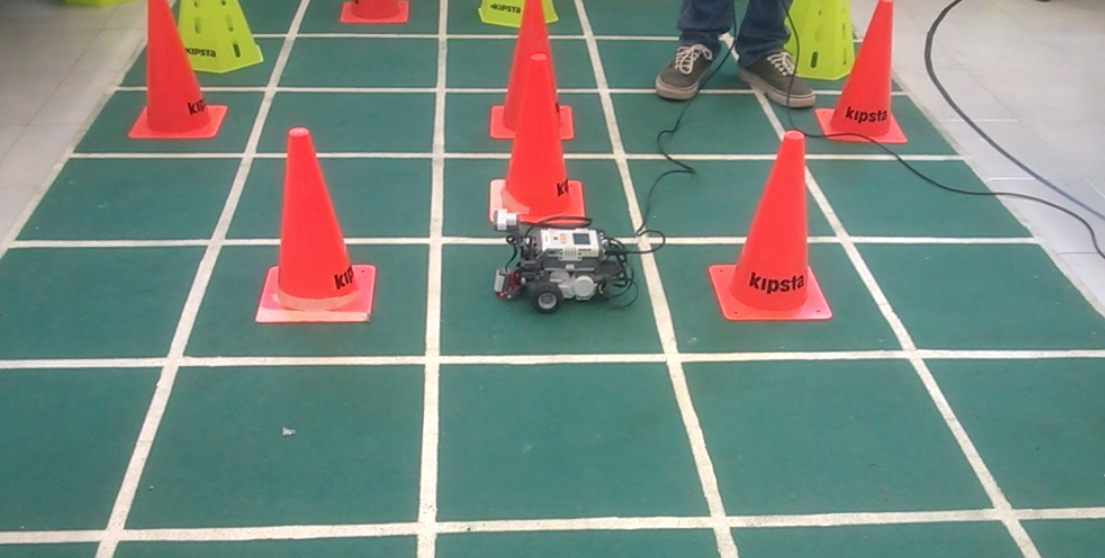
\includegraphics[width=0.4\textwidth,height=0.2\textwidth]{start}
\label{fig:start}}
\subfloat[Ricerca degli ostacoli - mappa a video.]	{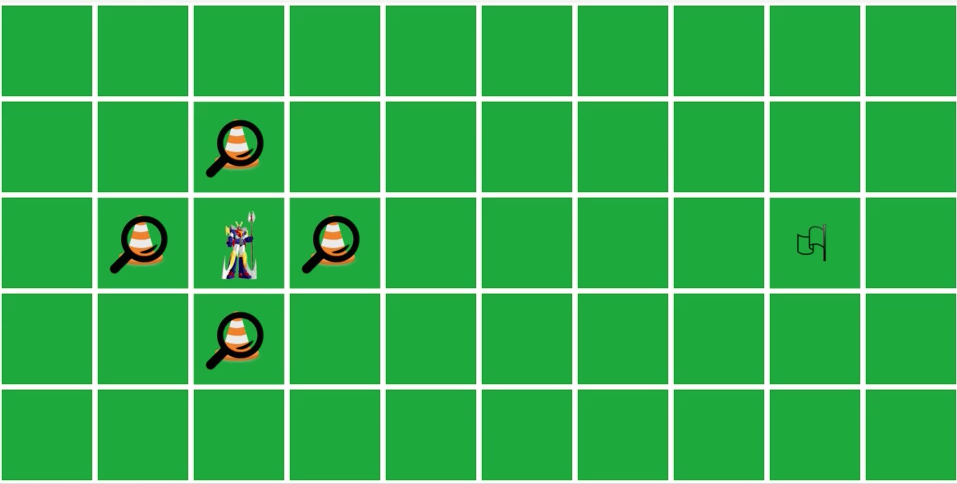
\includegraphics[width=0.4\textwidth,height=0.2\textwidth]{findostacolo}
\label{fig:findostacolo}}
\caption{Robot in posizione iniziale.}
%\label{fig: PzPs}
\end{figure}
\item A questo punto il robot trova che l'unica cella priva di ostacolo, è quella alla sua sinistra, quindi a video, il software visualizza la posizione degli ostacoli trovati all'interno della mappa (Figura \ref{fig:findostacolo}); ora il robot può ruotare in direzione Ovest, e procedere per avanzare nella cella successiva (Figura \ref{fig:passo1}).
\begin{figure}[!ht]
\centering
\subfloat[Robot che da posizione \textit{Start}, si muove verso Ovest.]	{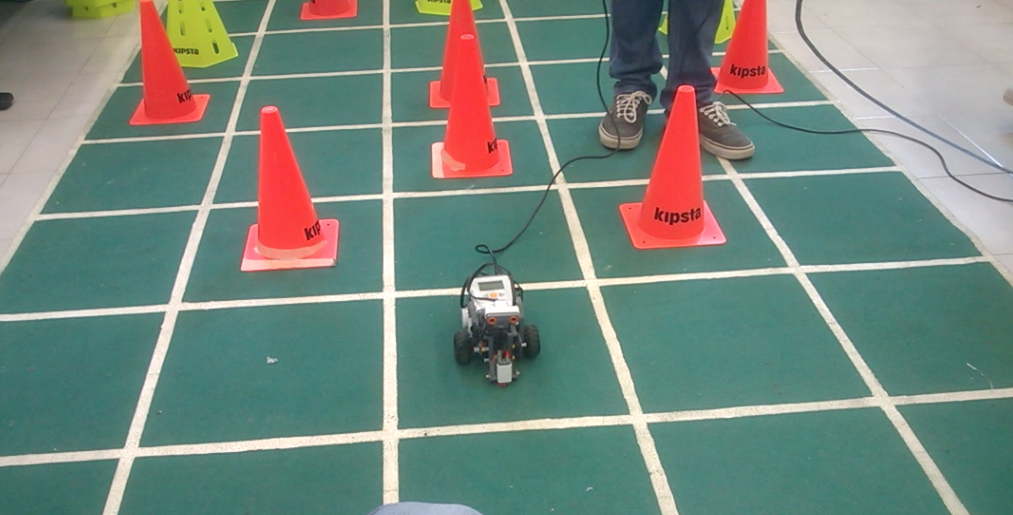
\includegraphics[width=0.4\textwidth,height=0.2\textwidth]{passo1}
\label{fig:passo1}}
\subfloat[Nella mappa viene mostrata l'intenzione del robot, di muoversi verso Ovest.]	{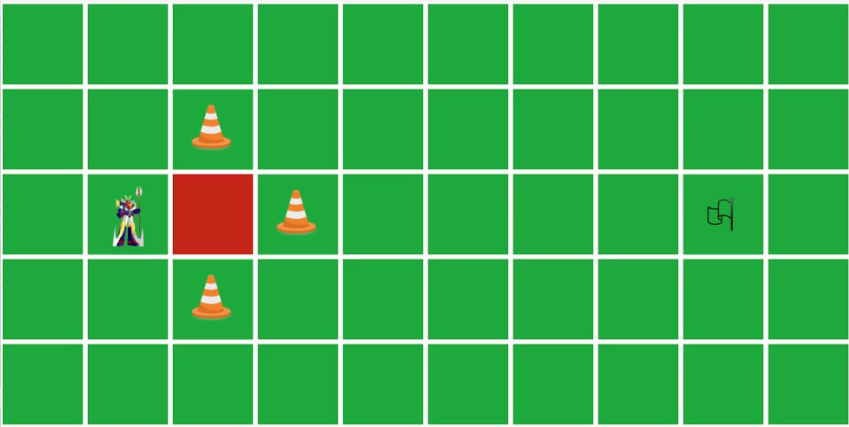
\includegraphics[width=0.4\textwidth,height=0.2\textwidth]{screen1}
\label{fig:screen1}}
\caption{Robot in movimento.}
%\label{fig: PzPs}
\end{figure}
\item Ora che il robot è giunto nella cella successiva, l'algoritmo ripete iterativamente le operazioni di ricerca ostacoli e calcolo del movimento successivo, finchè il robot non raggiunge la cella \textit{Goal}.
\end{enumerate}
Alla fine dell'algoritmo iterativo, il robot è finalmente giunto nella cella finale (Figura \ref{fig:goal}) e nella mappa grafica viene mostrato l'intero percorso valutato passo dopo passo dal robot (Figura \ref{fig:screen_goal}). 
\begin{figure}[!ht]
\centering
\subfloat[Robot che ha raggiunto la posizione finale.]	{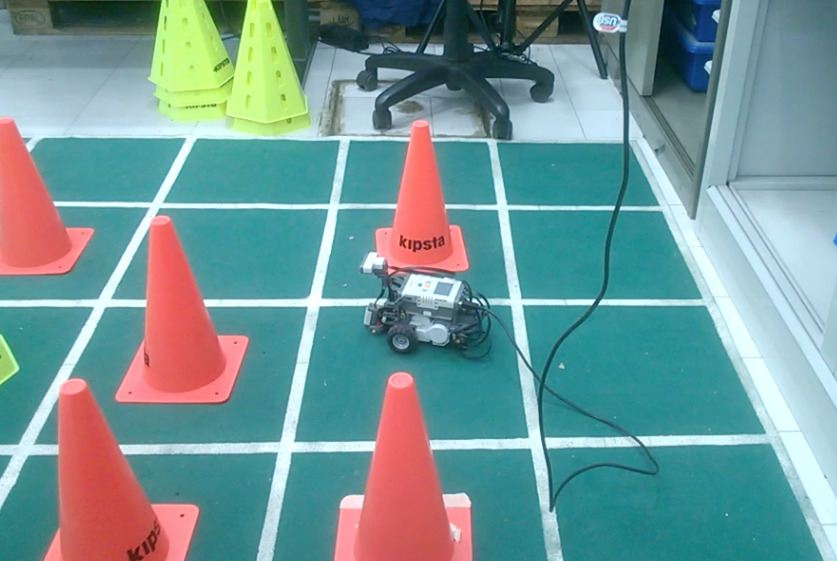
\includegraphics[width=0.4\textwidth,height=0.2\textwidth]{goal}
\label{fig:goal}}
\subfloat[Nella mappa viene mostrato l'intero percorso svolto dal robot, con i relativi ostacoli individuati.]	{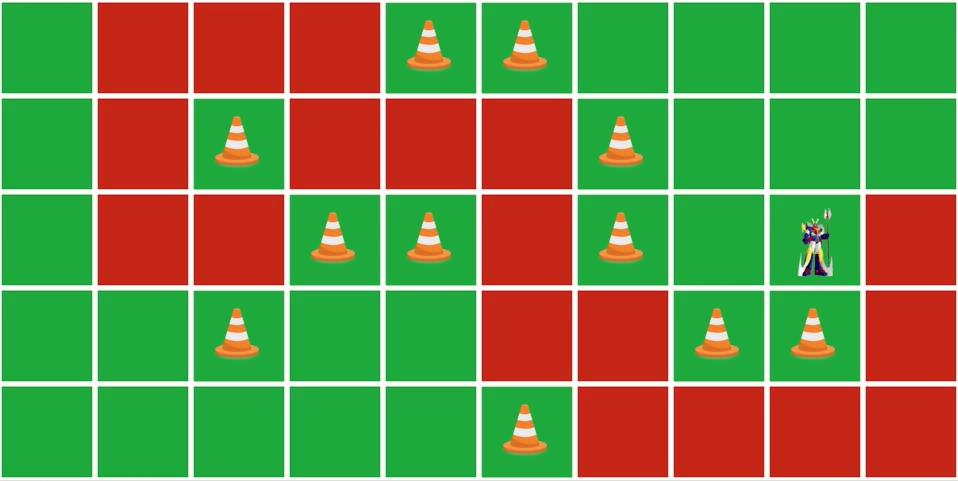
\includegraphics[width=0.4\textwidth,height=0.2\textwidth]{screen_goal}
\label{fig:screen_goal}}
\caption{Robot in posizione finale.}
%\label{fig: PzPs}
\end{figure}

\subsection{Scenario con ostacoli mobili}
Abbiamo visto come l'algoritmo di navigazione in questa ultima sezione, sia robusto a variazioni sulla mappa, in quanto questo non richiede che la mappa sia a priori nota. Una ulteriore complicazione all'algoritmo è possibile aggiungerla facendo si che la mappa cambi nel tempo. Supponiamo ad esempio che, ad un fissato istante temporale, il robot non trovi un percorso per arrivare al Goal. Con le ipotesi precedenti però, si prende in considerazione il fatto che, in un altro istante temporale successivo, la mappa cambi e si crei un percorso per arrivare alla fine. In queste ipotesi il robot è costretto, dopo un certo intervallo temporale, a ripetere l'operazione di ricerca degli ostacoli, per accertarsi di eventuali cambiamenti intercorsi. Di seguito dunque, si propone proprio tale scenario, in cui il robot viene chiuso all'interno di un percorso senza uscita, e ad un certo istante temporale, viene aperta una strada verso l'obiettivo finale.
\begin{figure}[!ht]
\centering
\subfloat[Robot senza strada per raggiungere il Goal.]	{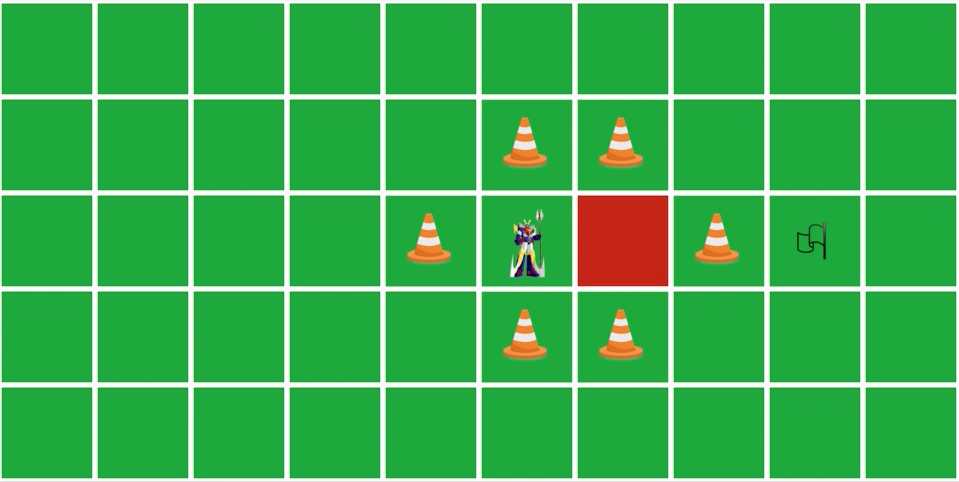
\includegraphics[width=0.4\textwidth,height=0.2\textwidth]{change_obstacles1}
\label{fig:change_obstacles1}}
\subfloat[Mappa dopo che il robot ha trovato uno spostamento degli ostacoli.]	{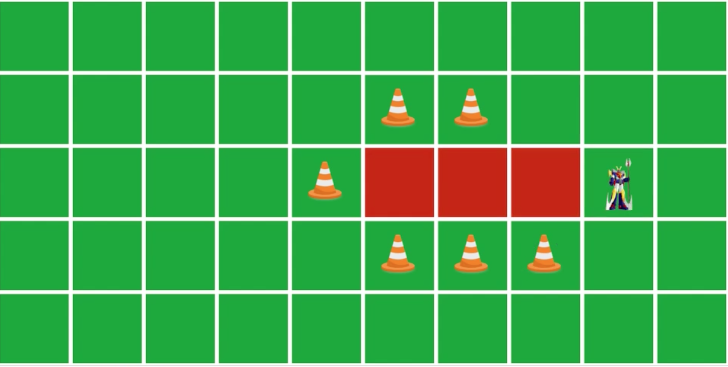
\includegraphics[width=0.4\textwidth,height=0.2\textwidth]{change_obstacles2}
\label{fig:change_obstacles2}}
\caption{Mappa prima e dopo lo spostamento dell'ostacolo.}
%\label{fig: PzPs}
\end{figure}
In Figura \ref{fig:change_obstacles1}, viene mostrato nella mappa come, all'inizio il robot continui a navigare all'interno di un percorso chiuso, e continui a trovare ostacoli nella stessa posizione di Prima. Figura \ref{fig:change_obstacles2} invece, mostra come, dopo lo spostamento di un ostacolo, il robot raggiunga ugualmente la cella finale.

\section{Conclusioni}
A conclusione di questa esperienza, si sono dunque raggiunti gli obiettivi di muovere il Lego-Nxt da una parte all'altra della mappa, utilizzando un'opportuno algoritmo per il calcolo del percorso. Quest'ultimo si basa sul sensore ad ultrasuoni, per il riconoscimento degli ostacoli, e sul sensore di luce per il riconoscimento dei quadrati nella griglia. Per la comunicazione con il robot Lego-Nxt si è fatto uso del software Ros, attivando attraverso un file launcher, 3 diversi nodi per la gestione della mappa, dei movimenti del robot, e dell'algoritmo di navigazione, ed è stato fatto uso dei topic di Ros per comunicare con i diversi sensori del robot. In seguito è stata data dimostrazione del funzionamento in laboratorio, in uno scenario in cui al robot venivano passate informazioni soltanto sulle celle di start, di goal, e sulle dimensioni della mappa, attraverso un file \textit{.yaml}. Una volta che sono stati posizionati gli ostacoli in diversi punti della mappa, si è osservato come il robot abbia correttamente riconosciuto questi ultimi, e sia riuscito a trovare un percorso per arrivare alla cella \textit{Goal}. In aggiunta, attraverso la libreria \textit{OpenCV} è stata creata una mappa, in grado di mostrare iterativamente a video i progressi del robot. 

Come ultima dimostrazione, si è voluto considerare il caso di mappa che cambia nel tempo, mettendo il robot in un circuito chiuso senza che abbia una possibilità di arrivare al goal. In questa situazione si è osservato come il robot, dopo non essere riuscito a trovare un percorso disponibile, continui a verificare se siano intercorsi cambiamenti nella mappa, anche tornando su strade già percorse. Infatti togliendo manualmente un ostacolo creando un percorso disponibile, in un certo istante di tempo, il robot se ne è accorto ed è potuto arrivare a destinazione. 


\clearpage

\end{document}